\secnumbersection{DEFINICIÓN DEL PROBLEMA}
\label{sec:def}

%=============================================================%
\subsection{Contexto} \label{sec:Contexto}
%=============================================================%
La gestión logística se ha consolidado como un pilar fundamental de la economía global, siendo determinante para la competitividad empresarial. En el año 2024, los costos logísticos comerciales en Estados Unidos alcanzaron los 2,6 billones de dólares, lo que representa aproximadamente el 8,8\% del PIB \footnote{El Producto Interno Bruto (PIB) corresponde al valor monetario total de los bienes y servicios finales producidos dentro de un país en un período determinado, y es utilizado comúnmente como indicador del tamaño y desempeño de una economía.} ~\cite{CSCMP2024}. Dicha cifra evidencia que la logística no es solo una función operativa, sino también una característica estructural de la economía moderna.

En tal escenario, la optimización del transporte adquiere un rol crítico. Diversas industrias como la gestión de residuos, la distribución de alimentos y los servicios de mantenimiento, entre muchas otras, enfrentan diariamente el desafío de planificar y gestionar rutas eficientes~\cite{UpperVRP}. De esta necesidad surge el Periodic Vehicle Routing Problem (PVRP), el cual busca diseñar rutas óptimas para una flota de vehículos que debe atender a clientes con una frecuencia específica dentro de un horizonte de planificación determinado, como semanal o mensual~\cite{EKSIOGLU20091472}. Este enfoque permite equilibrar la carga de trabajo y mejorar la eficiencia operativa a largo plazo.

No obstante, la complejidad inherente a tales problemas ha superado la capacidad de los métodos de planificación tradicional ante la volatilidad del mercado actual. Como resultado, la industria logística está experimentando una acelerada transformación tecnológica. De acuerdo con el reporte de tendencias tecnológicas para 2025 de Gartner, las cadenas de suministro están evolucionando hacia el uso de Agentic AI y técnicas de Reinforcement Learning, las cuales permiten la toma de decisiones autónomas y adaptativas frente a interrupciones, superando las limitaciones y la rigidez de las heurísticas clásicas~\cite{Gartner2025}.

%=============================================================%
\subsection{Motivación} \label{sec:Motivacion}
%=============================================================%
A pesar de los avances en métodos de optimización, la resolución de variantes complejas como el Periodic Vehicle Routing Problem (PVRP) continúa representando un desafío significativo. En escenarios reales, las empresas deben enfrentar condiciones operativas cambiantes, tales como variaciones en la demanda, interrupciones o modificaciones en el entorno logístico. Estas características hacen que la planificación de rutas no solo muestre eficiencia computacional, sino también capacidad de adaptación.

Tradicionalmente, este tipo de problemas ha sido abordado mediante heurísticas y metaheurísticas, las cuales buscan obtener soluciones de buena calidad en tiempos computacionales razonables. Entre los enfoques más utilizados se encuentran métodos basados en búsquedas locales, algoritmos evolutivos y técnicas como Variable Neighborhood Search (VNS)~\cite{HEMMELMAYR2009791}. Si bien estos métodos han demostrado ser efectivos, su desempeño depende en gran medida de las suposiciones y configuraciones bajo las cuales fueron diseñados.

Diversos estudios han identificado limitaciones en estos enfoques cuando se aplican a entornos dinámicos. En primer lugar, muchas heurísticas operan bajo reglas fijas predefinidas, lo que dificulta su adaptación frente a cambios inesperados en el entorno operativo, requiriendo frecuentemente procesos completos de reoptimización~\cite{nazari2018reinforcementlearningsolvingvehicle}. En segundo lugar, la calidad de las soluciones obtenidas suele depender fuertemente de la calibración de múltiples parámetros del algoritmo, cuya configuración adecuada puede resultar compleja y propensa al error humano~\cite{Chen,inproceedings}. Finalmente, algunos algoritmos constructivos presentan un comportamiento miope, priorizando decisiones locales logrando beneficios inmediatos pero sin considerar necesariamente su impacto global en el horizonte completo de planificación~\cite{inbook}.

Tales limitaciones evidencian la necesidad de explorar enfoques que permitan mejorar la capacidad adaptativa de los sistemas de planificación logística. Frente a este panorama, el Aprendizaje por Refuerzo (RL) ha emergido como una alternativa prometedora, ya que permite que un agente aprenda políticas de decisión directamente a partir de la interacción con el entorno, en lugar de depender exclusivamente de reglas creadas manualmente~\cite{SuttonBarto2014}. Lo anterior abre la posibilidad de desarrollar modelos capaces de adaptarse a diferentes instancias del problema y responder de forma más flexible a las condiciones cambiantes propias de los sistemas logísticos.

%=============================================================%
\subsection{Variantes relacionadas} \label{sec:Variantesrelacionadas}
%=============================================================%

El estudio del Vehicle Routing Problem (VRP) y sus variantes constituye un área consolidada y ampliamente documentada dentro de la optimización combinatoria, abordando diferentes configuraciones como el Capacitated Vehicle Routing Problem (CVRP) y el Vehicle Routing Problem with Time Windows (VRPTW)\cite{Casas}. Tradicionalmente, estos problemas han sido resueltos mediante heurísticas y metaheurísticas diseñadas para escenarios estáticos o de un solo periodo. Sin embargo, al extender el horizonte de planificación, como ocurre en el Periodic Vehicle Routing Problem (PVRP), el problema adquiere una complejidad adicional, ya que no sólo se deben determinar las rutas de los vehículos, sino también definir previamente el patrón de días en que cada cliente será atendido. Las implicancias de esta doble decisión sobre la complejidad computacional se analizan en detalle en la Sección \ref{sec:Complejidaddelproblema} ~\cite{EKSIOGLU20091472, inbook, HEMMELMAYR2009791}.

En respuesta a estas dificultades, diversos enfoques han sido propuestos en la literatura. Entre ellos, destacan las metaheurísticas como Variable Neighborhood Search (VNS), que han demostrado ser efectivas para explorar el espacio de soluciones del PVRP \cite{HEMMELMAYR2009791}. No obstante, estos métodos dependen fuertemente de reglas diseñadas manualmente y de una meticulosa calibración de parámetros, lo que limita su capacidad de adaptación a entornos dinámicos. Más recientemente, el uso de técnicas de aprendizaje automático, y en particular del Aprendizaje por Refuerzo (RL), ha emergido como una alternativa prometedora. Trabajos como el de Nazari et al.~\cite{nazari2018reinforcementlearningsolvingvehicle} han demostrado la capacidad de estos enfoques para aprender políticas de ruteo de manera intrínseca, construyendo soluciones de forma secuencial sin depender de reglas explícitas.

No obstante, si bien el Aprendizaje por Refuerzo ha mostrado resultados prometedores en ruteo estático, su aplicación a variantes temporales más complejas como el PVRP aún es un área incipiente y presenta importantes desafíos. Las investigaciones actuales carecen de modelos consolidados que aborden de manera conjunta la asignación de días y la creación de rutas periódicas mediante agentes autónomos, lo que motiva directamente la investigación y propuesta de solución presentada en esta memoria.

%=============================================================%
\subsection{Complejidad del problema} \label{sec:Complejidaddelproblema}
%=============================================================%
Como se mencionó previamente, el Periodic Vehicle Routing Problem (PVRP) se inscribe en la familia de problemas de optimización combinatoria conocidos como Vehicle Routing Problems (VRP). Estos han sido ampliamente estudiados en la investigación de operaciones dada su gran relevancia en aplicaciones logísticas reales. Su objetivo principal es determinar la planificación óptima de rutas para una flota de vehículos destinada a atender a un conjunto de clientes, minimizando el costo total de transporte bajo el cumplimiento de restricciones operacionales.

Desde el punto de vista computacional, el PVRP es clasificado como un problema NP-hard, lo que implica que no se conocen algoritmos capaces de encontrar soluciones óptimas en tiempo polinomial para todas las instancias del problema. Su complejidad surge de la naturaleza combinatoria del espacio de soluciones, el cual crece de manera exponencial a medida que aumenta el número de clientes, vehículos o periodos considerados en el horizonte de planificación~\cite{inbook}.

En el caso del PVRP, esta dificultad resalta por la incorporación de un horizonte temporal. A diferencia del VRP clásico, donde los clientes son atendidos en una única instancia, el PVRP exige determinar simultáneamente la asignación de los días de visita y las rutas a ejecutar en cada periodo. Esta doble decisión amplía de forma significativa el espacio de búsqueda, aumentando la complejidad computacional del problema~\cite{EKSIOGLU20091472}.

Como consecuencia, los métodos de programación matemática resultan inviables para instancias de gran tamaño, ya que el tiempo de cómputo requerido crece rápidamente con el tamaño del problema. Por esta razón, se ha recurrido al desarrollo de heurísticas y metaheurísticas capaces de obtener soluciones de buena calidad en tiempos computacionales razonables, aunque sin garantizar el óptimo global.

%=============================================================%
\subsection{Definición del problema} \label{sec:Definiciondelproblema}
%=============================================================%
El Periodic Vehicle Routing Problem (PVRP), introducido originalmente por Beltrami y Bodin~\cite{BeltramiBodin}, surge de la necesidad de planificar rutas a lo largo de un horizonte temporal para satisfacer la demanda de clientes que requieren múltiples visitas. 

Matemáticamente, el problema se define sobre un horizonte temporal de planificación $T = \{1, 2, \dots, t\}$ días. Se modela utilizando un grafo completo dirigido $G = (V, A)$, donde $V = \{0, 1, \dots, N\}$ es el conjunto de nodos, donde el nodo $\{0\}$ representa el depósito y el resto de nodos, $V' = \{1, \dots, N\}$, corresponden a los clientes. El conjunto de arcos $A = \{(i,j) : i,j \in V, i \neq j\}$ representa las conexiones entre los nodos, donde cada arco $(i,j)$ tiene asociado un costo de viaje $c_{ij}$. Se dispone de un conjunto de vehículos $K$, cada uno con una capacidad máxima $Q$. Cada cliente $i \in V'$ tiene asociada una demanda $q_{i}$ constante por visita y una frecuencia de visitas requerida $f_{i}$ dentro del horizonte $T$. Para satisfacer dicha frecuencia, cada cliente tiene un conjunto de combinaciones válidas de días de visita permitidos, denotado como $C_{i}$.

La solución al PVRP consiste en seleccionar exactamente una combinación de días $p \in C_{i}$ para cada cliente $i$, y simultáneamente construir un conjunto de rutas para cada vehículo $k \in K$ en cada día $d \in T$, tal que:
\begin{itemize}
    \item Todas las rutas comiencen y terminen en el depósito.
    \item Cada cliente sea visitado exactamente en los días estipulados por su combinación elegida.
    \item La demanda total de los clientes visitados por un vehículo en un solo día no excede su capacidad $Q$.
    \item Se minimice el costo total de las rutas a lo largo de todo el horizonte temporal.
\end{itemize}

\subsubsection{Ejemplo ilustrativo}
Para ilustrar el problema de forma más clara, imaginemos una empresa distribuidora de bebidas que planifica sus rutas en un horizonte temporal de 3 días ($T = \{\text{Lunes}, \text{Martes}, \text{Miércoles}\}$). La empresa cuenta con 2 camiones, cada uno con una capacidad máxima de $Q = 50$ unidades, y atiende a dos clientes con las siguientes características:

\begin{itemize}
    \item \textbf{Cliente A:} Demanda de $q_A = 30$ unidades por visita. Requiere $2$ visitas en el horizonte ($f_A = 2$). 
    
    \item \textbf{Cliente B:} Demanda de $q_B = 30$ unidades por visita. Requiere $1$ visita en el horizonte ($f_B = 1$). 
\end{itemize}

Una solución factible al problema requiere definir, en una primera etapa, la asignación temporal correspondiente, por ejemplo: visitar al Cliente A los días lunes y miércoles, y al Cliente B el lunes. En segundo lugar, se deben generar las rutas espaciales óptimas para cada camión en cada uno de dichos días, asegurando que el peso de las bebidas demandadas no supere la capacidad del camión asignado, minimizando los kilómetros totales recorridos al final de los tres días. La Figura \ref{fig:ejemplo_pvrp} ilustra la configuración espacial y temporal de esta solución óptima.

\begin{figure}[hbt!]
\centering
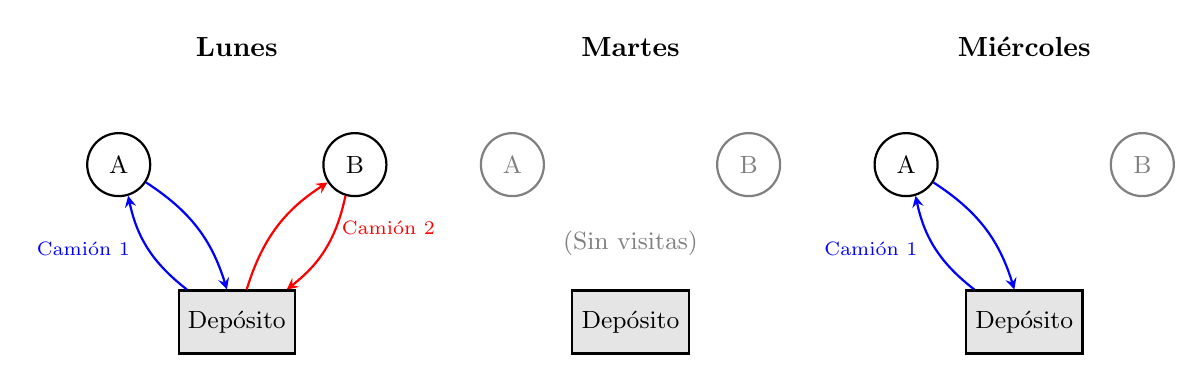
\begin{tikzpicture}[
    node distance=2cm,
    depot/.style={rectangle, draw=black, thick, fill=gray!20, minimum size=8mm, font=\small},
    client/.style={circle, draw=black, thick, fill=white, minimum size=8mm, font=\small},
    truck1/.style={->, thick, blue, >=stealth},
    truck2/.style={->, thick, red, >=stealth},
]
% LUNES
\begin{scope}[xshift=0cm]
    \node at (0, 3.5) {\textbf{Lunes}};
    \node[depot] (D1) at (0,0) {Depósito};
    \node[client] (A1) at (-1.5, 2) {A};
    \node[client] (B1) at (1.5, 2) {B};   
    % Rutas Lunes
    \draw[truck1] (D1) to[bend left=20] node[left, font=\scriptsize, xshift=-0.1cm] {Camión 1} (A1);
    \draw[truck1] (A1) to[bend left=20] (D1);
    \draw[truck2] (D1) to[bend left=20] node[right, font=\scriptsize, xshift=0.7cm] {Camión 2} (B1);
    \draw[truck2] (B1) to[bend left=20] (D1);
\end{scope}
% MARTES
\begin{scope}[xshift=5cm]
    \node at (0, 3.5) {\textbf{Martes}};
    \node[depot] (D2) at (0,0) {Depósito};
    \node[client, draw=gray, text=gray] (A2) at (-1.5, 2) {A};
    \node[client, draw=gray, text=gray] (B2) at (1.5, 2) {B};
    \node[font=\small, text=gray] at (0, 1) {(Sin visitas)};
\end{scope}
% MIERCOLES
\begin{scope}[xshift=10cm]
    \node at (0, 3.5) {\textbf{Miércoles}};
    \node[depot] (D3) at (0,0) {Depósito};
    \node[client] (A3) at (-1.5, 2) {A};
    \node[client, draw=gray, text=gray] (B3) at (1.5, 2) {B};
    \draw[truck1] (D3) to[bend left=20] node[left, font=\scriptsize, xshift=-0.1cm] {Camión 1} (A3);
    \draw[truck1] (A3) to[bend left=20] (D3);
\end{scope}
\end{tikzpicture}
\caption{\label{fig:ejemplo_pvrp}Representación de la solución óptima del PVRP para el ejemplo ilustrativo.}
Fuente: Elaboración propia.
\end{figure}


%=============================================================%
\subsubsection{Modelo Matemático} \label{sec:ModeloMatematico}
Para formular matemáticamente el Problema de Ruteo de Vehículos Periódico (PVRP), se sigue la estructura propuesta en~\cite{Coene2010}, donde se integran decisiones de asignación temporal y ruteo vehicular.

Sea $G = (V, A)$ un grafo dirigido, donde:
\begin{itemize}
    \item $V = \{0, 1, 2, ..., N\}$ es el conjunto de nodos, donde $0$ representa el depósito y $1,...,N$ los clientes.
    \item $A$ es el conjunto de arcos.
\end{itemize}

Se define un horizonte de planificación $T = \{1, ..., T\}$ días y un conjunto de vehículos $K$.

Cada cliente $i \in V'$ posee:
\begin{itemize}
    \item Una frecuencia de visita $f_i$,
    \item Una demanda $q_i$.
\end{itemize}

Se define un conjunto de combinaciones de días $C$, donde cada combinación $c \in C$ corresponde a un subconjunto de días del horizonte.

\textbf{Variables de decisión}

\begin{itemize}
    \item \textbf{Variable de ruteo:}
\[
x_{ijkt} =
\begin{cases}
1, & \text{si el vehículo } k \text{ viaja desde } i \text{ a } j \text{ en el día } t \\
0, & \text{en caso contrario}
\end{cases}
\]

    \item \textbf{Variable de asignación de patrón:}
\[
y_{ic} =
\begin{cases}
1, & \text{si el cliente } i \text{ es asignado al patrón } c \\
0, & \text{en caso contrario}
\end{cases}
\]
\end{itemize}

La función objetivo minimiza el costo total de transporte en el horizonte:

\begin{equation}
\min \sum_{i \in V} \sum_{j \in V} \sum_{k \in K} \sum_{t \in T} d_{ij} x_{ijkt}
\end{equation}

Sujeto a:

\textbf{Asignación de patrón:}
\begin{equation}
\sum_{c \in C: f_c = f_i} y_{ic} = 1 \quad \forall i \in V'
\end{equation}

\textbf{Consistencia entre patrón y visitas:}
\begin{equation}
\sum_{j \in V} \sum_{k \in K} x_{ijkt} = \sum_{c \in C} a_{ct} y_{ic} \quad \forall i \in V', \forall t \in T
\end{equation}

donde $a_{ct} = 1$ si el día $t$ pertenece al patrón $c$, y 0 en caso contrario.

\textbf{Conservación de flujo:}
\begin{equation}
\sum_{i \in V} x_{ihkt} = \sum_{j \in V} x_{hjkt} \quad \forall h \in V, \forall k \in K, \forall t \in T
\end{equation}

\textbf{Salida desde el depósito:}
\begin{equation}
\sum_{j \in V'} x_{0jkt} \leq 1 \quad \forall k \in K, \forall t \in T
\end{equation}

\textbf{Capacidad vehicular:}
\begin{equation}
\sum_{i \in V'} q_i \sum_{j \in V} x_{ijkt} \leq Q_k \quad \forall k \in K, \forall t \in T
\end{equation}

\textbf{Eliminación de subrutas:}
\begin{equation}
\sum_{i \in S} \sum_{j \in S} x_{ijkt} \leq |S| - 1 \quad \forall S \subseteq V', |S| \geq 2, \forall k \in K, \forall t \in T
\end{equation}

\textbf{Dominio de variables:}
\begin{equation}
x_{ijkt} \in \{0,1\}, \quad y_{ic} \in \{0,1\}
\end{equation}

A continuación se presentan los objetivos de este trabajo de memoria.

%=============================================================%
\subsection{Objetivo General} \label{sec:ObjetivoGeneral}
Desarrollar y evaluar un modelo basado en Aprendizaje por Refuerzo para la resolución del PVRP, con el fin de determinar políticas de ruteo eficientes y adaptativas.

\subsubsection{Objetivos Específicos}
\begin{enumerate}
    \item Analizar el estado del arte de las técnicas de optimización para el PVRP y las aplicaciones de Aprendizaje por Refuerzo en problemas de ruteo.
    \item Crear un entorno de simulación que modele adecuadamente las características y restricciones del PVRP.
    \item Crear un agente de Aprendizaje por Refuerzo funcional que sea capaz de interactuar con el entorno PVRP simulado y completar un ciclo de entrenamiento.
    \item Evaluar el modelo entrenado ejecutándose sobre un conjunto de instancias de PVRP, midiendo el costo total de las rutas generadas para cuantificar la diferencia respecto a los mejores resultados conocidos ~\cite{NEO2013}. 
    \item Comparar los resultados obtenidos por el modelo de RL con los de otros métodos de resolución reportados, incluyendo tanto una heurística simple como el algoritmo Greedy, así como un acercamiento ad-hoc del estado del arte, tal como la Búsqueda de Entorno Variable (VNS).
\end{enumerate}
